%!TEX root = paper.tex
%\section{Experimental Evaluation}

\newcommand{\ut}{untrustworthy\xspace}
\newcommand{\Ut}{Untrustworthy\xspace}


\ignore{
We now present experimental evaluation to demonstrate the effectiveness of data
\invariants (\system) in two major application areas: trusted machine learning
(Section~\ref{exp-invariants-for-ML}) and data-drift quantification
(Section~\ref{exp-invariants-for-drift}). We start by describing the
datasets and proceed to describe the results.
}

We now present experimental evaluation to demonstrate the effectiveness of \dis over our two case-study applications
(Section~\ref{sec:casestudies}): trusted machine learning and data drift.
Our experiments target the following research questions:     

\begin{itemize}
    \item How effective are \dis for trusted machine learning?
    Is there a relationship between \invariant violation score and the ML model's
    prediction accuracy? (Section~\ref{exp-invariants-for-ML})

    \item Can \dis be used to quantify data drift? How do they
    compare to other state-of-the-art drift-detection techniques?
    (Section~\ref{exp-invariants-for-drift})
    

    %
    % \item[{[RQ3]}] Can \dis be used to explain the causes for tuple
    % non-conformance? (Section~\ref{sec:extune})

\end{itemize}

% We now present experimental results to evaluate the efficacy of \dis
% (DI) on two applications. The research questions we aim to answer are:\\
%

\smallskip \noindent\textbf{Efficiency.} In all our experiments, our algorithms
for deriving \dis were extremely fast, and took only a few seconds even for
datasets with 6 million rows. The number of attributes were reasonably small
($\sim$40), which is true for most practical applications. As our theoretical
analysis showed (Section~\ref{sec:complexity}), our approach is linear in
the number of data rows and cubic in the number of attributes. Since the runtime
performance of our techniques is straightforward, we opted to not include
further discussion of efficiency here and instead focus this empirical analysis
on the techniques' effectiveness.


% Since we theoretically show the efficiency and scalability
% aspects of our approach (Section~\ref{sec:complexity}), we exclude empirical
% results to demonstrate those aspects. However, in our experiments, learning
% \dis were extremely fast and took only several seconds even for
% datasets with 6 million rows (our approach is linear in number of data rows).
% In all our experiments, the number of attributes were reasonably small
% ($\sim$40), which is true for most practical applications (our approach is
% cubic in number of attributes).

\smallskip
\noindent 
\textbf{Implementation: \system.} 
%
We created an implementation of \dis and our method for synthesizing them,
\system, in Python 3~\cite{diSource}. Experiments were run on a Windows 10
machine (3.60 GHz processor and 16GB RAM).




%
% \subsection{Experimental Setup}
% %
% In this section, we discuss the baseline approaches we compare \system against,
% and the datasets we use in the experiments.
%
%
\smallskip
\noindent
{\large \textit{Datasets}}
\smallskip
%
% \noindent\textbf{Synthetic Datasets.} We use a toy dataset and a synthetic
% benchmark for our experiments and we describe them below:
%
% \smallskip
%
% \emph{TOY.} This is a toy dataset which we synthetically generated. The dataset
% contains four numerical attributes: $x_1, x_2, x_3$, and $x_4$. Each attribute is
% sampled from a normal distribution. The task we design on this dataset is to
% learn a Boolean function to detect whether $x_1 + x_2$ is greater than $x_3 +
% x_4$, i.e., $\mathbbm{1}(x_1 + x_2 > x_3 + x_4)$. We use this dataset for
% experiments in the trusted machine learning problem setting.

%\smallskip

%\smallskip

\noindent\textbf{Airlines}~\cite{airlineSource} contains data about
flights and has 14 attributes
%, such as departure and arrival time, carrier, delay, etc.
\reviseone{---year, month, day, day of week, departure time, arrival time,
carrier, flight number, elapsed time, origin, destination, distance, diverted,
and arrival delay.}
% 
We used a subset of the data containing all flight information for year 2008.
\reviseone{In this dataset, most of the attributes follow uniform distribution
(e.g., month, day, arrival and departure time, etc.); elapsed time and distance
follow skewed distribution with higher concentration towards small values
(implying that shorter flights are more common); arrival delay follows a
slightly skewed gaussian distribution implying most flights are on-time, few
arrive late and even fewer arrive early.}
% and apply label encoding to convert the categorical
% attributes (e.g., carrier) to numerical attributes. 
The training and serving datasets contain 5.4M and 0.4M rows, respectively.
% We use this dataset for a regression task of predicting the
% arrival delay in the trusted machine learning problem setting.

\smallskip

%
% \noindent\textbf{Real Datasets.} We use two real-world datasets in our
% experiments and we describe them below:
%
% \smallskip

\noindent \looseness-1 \textbf{Human Activity Recognition
(HAR)}~\cite{sztyler2016onbody} is a real-world dataset about physical
activities for 15 individuals, 8 males and 7 females, with varying fitness
levels and BMIs. We use data from two sensors---accelerometer and
gyroscope---attached to 6 body locations---head, shin, thigh, upper arm, waist,
and chest. We consider 5 activities---lying down, running, sitting, standing,
and walking. The dataset contains 36 numerical attributes (2 sensors $\times$ 6
body-locations $\times$ 3 co-ordinates) and 2 categorical
attributes---activity-type and person-ID. We pre-processed the dataset to
aggregate the measurements over a small time window, resulting in 10,000 tuples
per person and activity, for a total of 750,000 tuples.


\smallskip

\noindent\textbf{Extreme Verification Latency (EVL)}~\cite{souzaSDM:2015}
%To test how effectively \system detects artificially induced
%drifts, we use an 
is a widely used benchmark to evaluate drift-detection algorithms in
non-stationary environments under extreme verification latency. It contains 16
synthetic datasets with incremental and gradual concept drifts over time. The
number of attributes of these datasets vary from 2 to 6 and each of them has
one categorical attribute.

\ignore{
\smallskip

\noindent\textbf{Datasets for non-conformance explanation case studies.}
\looseness-1 We evaluate the effectiveness of \dis in explaining tuple
non-conformance through an intervention-centric explanation tool built on top
of \system, called
\extune~\cite{DBLP:conf/sigmod/FarihaTRG20}. We use four datasets for this evaluation:
(1)~\emph{Cardiovascular Disease}~\cite{cardioSource} is a real-world dataset
that contains information about cardiovascular patients with attributes such as
height, weight, cholesterol level, glucose level, systolic and diastolic blood
pressures, etc. (2)~\emph{Mobile Prices}~\cite{mobilePriceSource} is a
real-world dataset that contains information about mobile phones with
attributes such as ram, battery power, talk time, etc. (3)~\emph{House
Prices}~\cite{housePriceSource} is a real-world dataset that contains
information about houses for sale with attributes such as basement area, number
of bathrooms, year built, etc. (4)~\emph{LED} (Light Emitting
Diode)~\cite{DBLP:journals/jmlr/BifetHKP10} is a synthetic benchmark. The
dataset has a digit attribute, ranging from 0 to 9, 7 binary attributes---each
representing one of the 7 LEDs relevant to the digit attribute---and 17
irrelevant binary attributes. This dataset includes gradual concept drift every
25,000 rows.
}
%
% \smallskip
%
% \emph{HousePrice.} House Prices~\cite{housePriceSource} is a dataset about
% house prices, originally aimed for the regression task of predicting sale price
% of the houses. The dataset consists of 79 attributes---36 among them are numeric.
% We only consider the numeric attributes in our experiments of
% \emph{responsibility assignment} on attributes for explaining drift in data.


% \smallskip

% \noindent \emph{MNIST.} MNIST~\cite{lecun1998gradient} is a very popular
% dataset for handwritten digit recognition. The raw dataset image size was
% 24$\times$24. We scaled down the images to 8$\times$8
% size and used the 64 pixel values as attributes.


\subsection{Trusted Machine Learning}\label{exp-invariants-for-ML}
%!TEX root = drift.tex
% \section{Experimental Evaluation}
% \subsection{Using \Invariants for Trusting Learnt Models}

\looseness-1 We now demonstrate the applicability of \dis in the TML problem.
We show that, serving tuples that violate the training data's \dis are \nc, and
therefore, an ML model is more likely to perform poorly on those tuples.


\smallskip

\begin{figure}[t!]
	\centering
	\setlength{\tabcolsep}{5pt}
	\renewcommand\arraystretch{0.88}
	\small{
	\begin{tabular}{ccccc}
		\hline
		&  \multirow{ 2}{*}{Train} & \multicolumn{3}{c}{Serving}\\
		\cline{3-5}
		&& Daytime & Overnight & Mixed \\
		\midrule
		\textbf{Average violation} & 0.02\% & 0.02\% & 27.68\% & 8.87\%\\
		\textbf{MAE} & 18.95	 &  18.89 & 80.54 & 38.60\\
		\bottomrule
		
	\end{tabular}
	}
		\vspace{-3mm}	
	 \caption{Average \invariant violation (in percentage) and MAE (for linear regression) 
	 of four data splits on the airlines dataset. The \invariants were learned on
 	 \texttt{Train}, excluding the target attribute, \texttt{delay}.}
	 
	\label{fig:airlines-summary}
	\vspace{2mm}
	\centering
	\includegraphics[width=0.75\linewidth]{Plots/Figure_5.pdf}
	\vspace{-3mm}	
	\caption{\Invariant violation strongly correlates with the absolute error
	 of delay prediction of a linear regression model.}
	 \vspace{2mm}	
	\label{fig:airlines}
\end{figure}


\noindent \textbf{Airlines.} We design a regression task of predicting the
arrival delay and train a linear regression model for the task. \reviseone{Our
goal is to observe whether the mean absolute error of the predictions
(positively) correlates to the \invariant violation for the serving tuples.} In
a process analogous to the one described in Example~\ref{ex:tml}, our training
dataset (\texttt{Train}) comprises of a subset of daytime flights---flights
that have arrival time later than the departure time (in 24 hour format). We
design three serving sets: (1)~\texttt{Daytime}: similar to \texttt{Train}, but
another subset, (2)~\texttt{Overnight}: flights that have arrival time earlier
than the departure time (the dataset does not explicitly report the date of
arrival), and (3)~\texttt{Mixed}: a mixture of \texttt{Daytime}
and~\texttt{Overnight}. \reviseone{A few sample tuples of this dataset are in
Fig.~\ref{fig:flights}.}

\reviseone{Our experiment involves the following steps: (1)~\system computes
\dis $\Phi$ over \texttt{Train}, while \emph{ignoring} the target attribute
\texttt{delay}. (2)~We compute average \invariant violation for all four
datasets---\texttt{Train}, \texttt{Daytime}, \texttt{Overnight}, and
\texttt{Mixed}---against $\Phi$ (first row of Fig.~\ref{fig:airlines-summary}).
(3)~We train a linear regression model over \texttt{Train}---including
\texttt{delay}---that learns to predict arrival delay. (4)~We compute mean
absolute error (MAE) of the prediction accuracy of the regressor over the four
datasets (second row of Fig.~\ref{fig:airlines-summary}).} We find
that \invariant violation is a very good proxy for prediction error, as they
vary in a similar manner across the four datasets. The reason is that the model
implicitly assumes that the \invariants (e.g., $AT - DT - DUR \approx 0$)
derived by \system will always hold, and, thus, deteriorates when the assumption
no longer holds.


\looseness-1 \reviseone{To observe the rate of false positives and false
negatives, we investigate the relationship between constraint violation and
prediction error at tuple-level granularity.} We sample 1000 tuples from
\texttt{Mixed} and organize them by decreasing order of violations
(Fig.~\ref{fig:airlines}). \reviseone{For all the tuples (on the left) that
incur high \invariant violations, the regression model incurs high error for
them as well. This implies that \system reports no false positives. There are some false negatives (right part of the graph), where violation is low, but
the prediction error is high. Nevertheless, such false negatives are very few.}

% \af{tofix}
% {	\footnotesize
% \begin{align*}
% -250 \le & 0.61	 {\cdot} dep {-}0.60 {\cdot} arr {+}  0.0 {\cdot} fno {+} 0.07 {\cdot} dur {+}  0.40 {\cdot} orig {-}  0.32 {\cdot} dest {+} 0.11 {\cdot} dist \le 360\\
% -280 \le & 0.34	 {\cdot} dep {-}0.34 {\cdot} arr {+}  0.0 {\cdot} fno {+} 0.04 {\cdot} dur {-}  0.50 {\cdot} orig {+}  0.72 {\cdot} dest {+} 0.05 {\cdot} dist \le 270\\
% \end{align*}
% }

 
\smallskip

\noindent\textbf{HAR.}
%
We design a supervised classification task to identify persons from their
activity data \reviseone{that contains 36 numerical attributes.} We construct
\texttt{train\_x} with data for sedentary activities (lying, standing, and
sitting), and \texttt{train\_y} with the corresponding person-IDs. We learn
\dis on \texttt{train\_x}, and train a Logistic Regression (LR) classifier
using the annotated dataset $[\texttt{train\_x};$ $\texttt{train\_y}]$. During
serving, we mix mobile activities (walking and running) with held-out data for
sedentary activities and observe how the classification's mean accuracy-drop
\reviseone{(i.e., how much the mean prediction accuracy decreases compared to
the mean prediction accuracy over the training data)} relates to average
\invariant violation. \reviseone{To avoid artifacts due to sampling bias, we
repeat this experiment $10$ times for different subsets of the data by randomly
sampling $5000$ data points for each of training and serving.}
Fig.~\ref{fig:har-ml-experiment}~depicts our findings: classification
degradation has a clear positive correlation with violation (pcc = 0.99 with
p-value = 0).

\smallskip

\looseness-1 \noindent \revisetwo{\emph{Noise sensitivity.} \label{noise}
Intuitively, noise weakens \dis by increasing variance in the training data,
which results in reduced violations of the serving data. However, this is
desirable: as more noise makes machine-learned models less likely to overfit,
and, thus, more robust. In our experiment for observing noise sensitivity of
\dis, we use mobile activity data as the serving set and start with sedentary
data as the training set. Then we gradually introduce noise in the training set
by mixing mobile activity data. As Fig.~\ref{fig:har-ml-experiment-noise}
shows, when more noise is added to the training data, \dis start getting
weaker; this leads to reduction in violations. However, the classifier also
gains robustness with more noise, which is evident from gradual decrease in
accuracy-drop (i.e., increase in accuracy). Therefore, even under the presence
of noise, the positive correlation between classification degradation and
violation persists (pcc = 0.82 with p-value = 0.002).}


\smallskip
\noindent
\fbox{
\parbox{0.96\columnwidth}{
\emph{Key takeaway:} 
%
\system derives \dis whose violation is a strong proxy of model prediction
accuracy. \reviseone{Their correlation persists even in the presence of noise.}}
%
}

\begin{figure}[t!]
	\centering
	\vspace{-3mm}
	\hspace{-3mm}
	\begin{subfigure}[t]{0.16\textwidth}
		\centering
		\includegraphics[width=\linewidth]{Plots/Figure_6_a.pdf}
	\vspace{-5mm}
	\caption{\phantom{randomrand}}
	\label{fig:har-ml-experiment}
	\end{subfigure}	
	\begin{subfigure}[t]{0.16\textwidth}
		\centering
		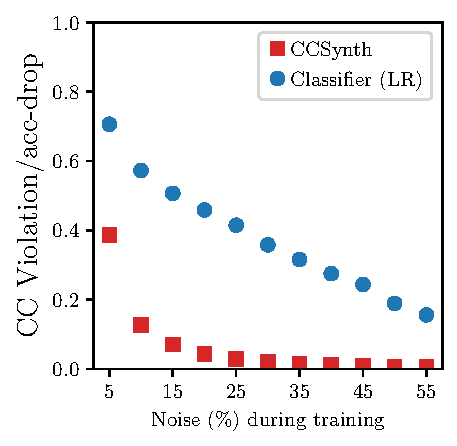
\includegraphics[width=\linewidth]{Plots/Figure_6_b.pdf}
	\vspace{-5mm}
	\caption{}
	\label{fig:har-ml-experiment-noise}
	\end{subfigure}	
	\begin{subfigure}[t]{0.16\textwidth}
		\centering
		\includegraphics[width=\linewidth]{Plots/Figure_6_c.pdf}
	\vspace{-5mm}
	\caption{}
	\label{fig:gradual-drift-har}
	\end{subfigure}
	\vspace{-5mm}	
	\caption{(a)~As a higher fraction of mobile activity data is mixed with
sedentary activity data, \dis are violated more, and the classifier's
mean accuracy-drop increases. 
%
(b)~\revisetwo{As more noise is added during training, \dis get weaker,
leading to less violation and decreased accuracy-drop.}
%
(c)~\system detects the gradual local drift on the
HAR dataset as more people start changing their
activities. In contrast, weighted-PCA (W-PCA) fails to detect drift in absence of
a strong global drift.} 
		\vspace{2mm}	
	\centering
	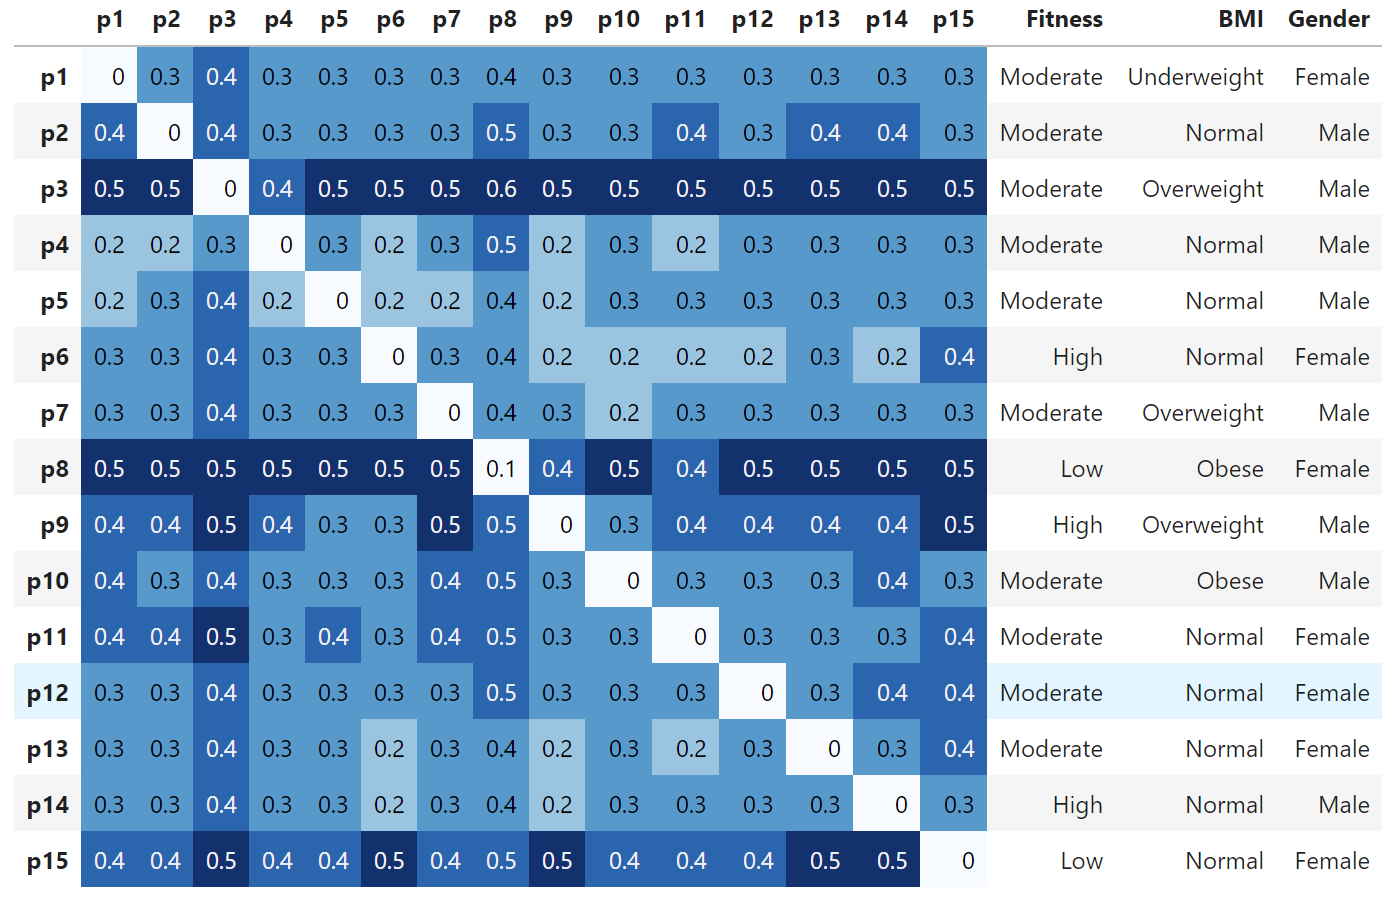
\includegraphics[width=1\linewidth]{Figures/Figure_7.png}
		\vspace{-7mm}	
	\caption{\looseness-1 Inter-person \invariant violation heat map. Each person has a very low self-violation.}
	\label{fig:har-inter-person-drift-heatmap}
		\vspace{1mm}	
	\centering
\end{figure}

\smallskip

\subsection{Data Drift}\label{exp-invariants-for-drift}
%
% \looseness-1
We now present results of using \dis for drift-detection; specifically, for
\emph{quantifying} drift in data. Given a baseline dataset $D$, and a new
dataset $D'$, we measure the drift as average violation of tuples in $D'$ on
\dis learned for $D$.

\smallskip

\noindent\textbf{HAR.} We perform two drift-quantification experiments on
HAR:

\smallskip

\noindent \emph{Gradual drift.} \looseness-1 For observing how \system detects
gradual drift, we introduce drift in an organic way. The initial training
dataset contains data of exactly one activity for each person. This is a
realistic scenario as one can think of it as taking a snapshot of what a group
of people are doing during a reasonably small time window. We introduce gradual
drift to the initial dataset by altering the activity of one person at a time.
To control the amount of drift, we use a parameter $K$. \reviseone{When $K =
1$, the first person switches their activity, i.e., we replace the tuples
corresponding to the first person performing activity A with new tuples that
correspond to the same person performing another activity B.} When $K = 2$, the
second person switches their activity in a similar fashion, and so on. As we
increase $K$ from $1$ to $15$, we expect a gradual increase in the drift
magnitude compared to the initial training data. When $K = 15$, all persons
have switched their activities from the initial setting, and we expect to
observe maximum drift. We repeat this experiment $10$ times, and display the
average \invariant violation in Fig.~\ref{fig:gradual-drift-har}: the drift
magnitude (violation) indeed increases as more people alter their activities.

\begin{figure*}[t]
	\centering	
	\includegraphics[width=.8\linewidth]{Plots/Figure_8.pdf}	
		\vspace{-5mm}
	 \caption{In the EVL benchmark, \system quantifies drift correctly for all
	 cases, outperforming other approaches. PCA-SPLL fails to detect drift in a few cases by
 	 discarding all principal components; CD-MKL and CD-Area are too sensitive to
 	 small drift and detect spurious drifts.}
	\vspace{-2mm}
	\label{fig:drift-baseline-comparison-EVL}
\end{figure*}

The baseline weighted-PCA approach (W-PCA) fails to model local \invariants
(who is doing what), and learns some weaker global \invariants indicating that
``a group of people are performing some activities''. Thus, it fails to detect
the gradual local drift. \system can detect drift when individuals switch
activities, as it learns \emph{disjunctive} \invariants that encode who is
doing what.

\smallskip


\noindent \looseness-1 \emph{Inter-person drift.} \reviseone{The goal of this
experiment is to observe how effectively \dis can model the representation of an
entity and whether such learned representations can be used to accurately
quantify drift between two entities.} We use half of each person's data to
learn the \invariants, and compute violation on the held-out data. \system
learns disjunctive \invariants for each person over all activities, and then we
use the violation w.r.t.\ the learned \invariants to measure how much the other
persons drift. While computing drift between two persons, we compute
activity-wise \invariant violation scores and then average them out. In
Fig.~\ref{fig:har-inter-person-drift-heatmap}, the violation score at row
\texttt{p1} and column \texttt{p2} denotes how much \texttt{p2} drifts from
\texttt{p1}. As one would expect, we observe a very low self-drift across the
diagonal. Interestingly, our result also shows that some people are more
different from others, which appears to have some correlation with (the hidden
ground truth) fitness and BMI values. This asserts that the \invariants we
learn for each person are an accurate abstraction of that person's activities,
as people do not deviate too much from their usual activity patterns.




\smallskip

\noindent \textbf{EVL.} We now compare \system against other state-of-the-art
drift detection approaches on the EVL benchmark.

\smallskip

\noindent\emph{Baselines.}
%
We use two drift-detection baselines as described below:

\smallskip

(1)~PCA-SPLL~\cite{DBLP:journals/tnn/KunchevaF14} 
%\footnote{\scriptsize{SPLL
%source code: }\scriptsize{\url{github.com/LucyKuncheva/Change-detection}}},
similar to us, also argues that principal components with lower variance are
more sensitive to a general drift, and uses those for dimensionality reduction.
It then models multivariate distribution over the reduced dimensions and
applies semi-parametric log-likelihood (SPLL) to detect drift between two
multivariate distributions. However, PCA-SPLL discards all high-variance
principal components and does not model disjunctive \invariants.

\smallskip
 
(2)~CD (Change Detection)~\cite{DBLP:conf/kdd/QahtanAWZ15}
%\footnote{\scriptsize{CD source code:}
%\scriptsize{\url{mine.kaust.edu.sa/Pages/Software.aspx}}} 
is another PCA-based approach for drift detection in data streams. But unlike
PCA-SPLL, it ignores low-variance principal components. CD projects the data
onto top $k$ high-variance principal components, which results into multiple
univariate distributions. We compare against two variants of CD: CD-Area, which
uses the intersection area under the curves of two density functions as a
divergence metric, and CD-MKL, which uses Maximum KL-divergence as a symmetric
divergence metric, to compute divergence between the univariate distributions.

\smallskip

\looseness-1 Fig.~\ref{fig:drift-baseline-comparison-EVL} depicts how \system
compares against CD-MKL, CD-Area, and PCA-SPLL, on 16 datasets in the
EVL benchmark. For PCA-SPLL, we retain principal components that contribute to
a cumulative explained variance below 25\%. Beyond drift detection, which just
detects if drift is above some threshold, we focus on drift
quantification. A tuple $(x,y)$ in the plots denotes that drift
magnitude for dataset at $x^{th}$ time window, w.r.t.\ the dataset at the first
time window, is $y$. Since different approaches report drift magnitudes in
different scales, we normalize the drift values within $[0, 1]$. Additionally,
since different datasets have different number of time windows,
for the ease of exposition, we normalize the time window indices. Below
we state our key findings from this experiment:
% in a similar way (determined by the data and
%window sizes). 

%  $\mathbf{c} = \{ c_0, \ldots, c_n\}$ within the
% range [0, 1] by using a simple transformation: $ \hat{c_i} = \frac{c_i -
% \min(\mathbf{c})} {\max(\mathbf{c}) - \min(\mathbf{c})}$.

\smallskip 

 
\looseness-1 \emph{\system's drift quantification matches the ground truth.} In
all of the datasets in the EVL benchmark, \system is able to correctly quantify
the drift, which matches the ground truth~\cite{evlVideo} exceptionally well.
In contrast, as CD focuses on detecting the drift point, it is ill-equipped to
precisely quantify the drift, which is demonstrated in several cases (e.g.,
2CHT), where CD fails to distinguish the deviation in drift magnitudes. In
contrast, both PCA-SPLL and \system correctly quantify the drift.
\revisetwo{Since CD only retains high-variance principal components, it is more
susceptible to noise and considers noise in the dataset as significant drift,
which leads to incorrect drift quantification. In contrast, PCA-SPLL and
\system ignore the noise and only capture the general notion of drift.}
% In all
% of the EVL datasets, we found CD-Area to work better than CD-MKL, which also
% agrees with the authors' experiments.


\smallskip

\looseness-1 \emph{\system models local drift.} When the dataset contains
instances from multiple classes, the drift may be just local, and not global
(e.g., 4CR dataset~\citeTechRep). In such cases, PCA-SPLL fails to detect drift
(4CR, 4CRE-V2, and FG-2C-2D). In contrast, \system learns disjunctive
\invariants and quantifies local drifts accurately.


\smallskip
\noindent
\fbox{
\parbox{0.95\columnwidth}{
\emph{Key takeaways:} 
%
\system can effectively detect data drift, both global and local, is robust
across drift patterns, and significantly outperforms the state-of-the-art
methods.}
%
}

\ignore{
\subsection{Explaining Non-conformance}\label{sec:extune}

When a serving dataset is determined to be sufficiently different or drifted
from the training set, the next step often is to characterize the difference. A
common way of characterizing these differences is to perform a causality or
responsibility analysis to determine which attributes are most responsible for
the observed drift (non-conformance). We use the violation values produced by
\dis, along with well-established principles of causality, to quantify
responsibility for non-conformance.

\smallskip 

\noindent\textbf{\extune.} \looseness-1 We built a tool
\extune~\cite{DBLP:conf/sigmod/FarihaTRG20}\footnote{Anonymized due to double
blind consideration.}, on top of \system, to compute the
responsibility values as described next. Given a training dataset $D$ and a
non-conforming tuple $t \in {\DDom}^m$, we measure the \emph{responsibility} of
the $i^{th}$ attribute $A_i$ towards the non-conformance as follows: (1)~We
intervene on $t.A_i$ by altering its value to the mean of $A_i$ over $D$ to
obtain the tuple $t^{(i)}$. (2)~In $t^{(i)}$, we compute how many additional
attributes need to be altered to obtain a tuple with no violation. If $K$
additional attributes need to be altered, $A_i$ has responsibility
$\frac{1}{K+1}$. (3)~This responsibility value for each tuple $t$ can be
averaged over the entire serving dataset to obtain an aggregate responsibility
value for $A_i$.
%
Intuitively, for each tuple, we are ``fixing'' the value of $A_i$ with a
``more typical'' value, and checking how close (in terms of additional fixes required) this takes us to a conforming tuple.
The larger the number of additional fixes required, the lower the responsibility of $A_i$.


\begin{figure}
	\centering
	%
	\begin{subfigure}{.09\textwidth}
	  \centering
	  \includegraphics[width=\linewidth, height=40mm]{Figures/cardio.pdf}
	  \caption{}
	  \label{cardio}
	\end{subfigure}
	\hspace{-1mm}
	\begin{subfigure}{.09\textwidth}
	  \centering
	  \includegraphics[width=\linewidth, height=40mm]{Figures/mobileprice.pdf}
	  \caption{}
	  \label{mobilePrice}
	\end{subfigure}
	\hspace{-1.5mm}
	\begin{subfigure}{.09\textwidth}
	  \centering
	  \includegraphics[width=\linewidth, height=40mm]{Figures/houseprice.pdf}
	  \caption{}
	  \label{housePrice}
	\end{subfigure}
	\hspace{-1.5mm}
	\begin{subfigure}{.2\textwidth}
		\centering
		\includegraphics[width=.9\linewidth, height=40mm]{Figures/LED-drift.pdf}
	  	\caption{}
	    \label{fig:LED-drift}
	\end{subfigure}
	\vspace{-3mm}
	%
	\caption{Responsibility assignment on attributes for drift on 
	(a)~Cardiovascular disease: trained on patients with no disease and served on patients with disease,
	(b)~Mobile Prices: trained on cheap mobiles and served on expensive mobiles and 
	(c)~House Prices: trained on house with price $<=$ 100K and served on house with price $>=$ 300K.
	(d)~Detection of drift on LED dataset. The dataset drifts every 5
		 windows (25,000 tuples). At each drift, a certain set of LEDs
		 malfunction and take responsibility of the drift.}
	\label{fig:extune}
	\vspace{-7mm}
\end{figure}

\begin{figure}
	\centering


\end{figure}

% Does the word intervenes have a special meaning? Do we need to retain it? 
\smallskip

\noindent\textbf{Case studies.} \extune produces bar-charts of responsibility
values as depicted in Fig.~\ref{fig:extune}.
Figures~\ref{cardio},~\ref{mobilePrice}, and~\ref{housePrice} show the
explanation results for Cardiovascular Disease, Mobile Price, and House Price
datasets, respectively. For the cardiovascular disease dataset, the training
and serving sets consist of data for patients without and with cardiovascular
disease, respectively. For the House Price and Mobile Price datasets, the
training and serving sets consist of houses and mobiles with prices below and
above a certain threshold, respectively. As one can guess, we get many useful
insights from the non-conformance responsibility bar-charts such as: ``abnormal
(high or low) blood pressure is a key cause for non-conformance of patients
with cardiovascular disease w.r.t. normal people'', ``RAM is a distinguishing
factor between expensive and cheap mobiles'', ``the reason for houses being
expensive depends holistically on several attributes''.

Fig.~\ref{fig:LED-drift} shows a similar result on the LED dataset. Instead
of one serving set, we had 20 serving sets (the first set is also used as a training
set to learn \dis). We call each serving set a window where each window
contains 5,000 tuples. This dataset introduces gradual concept drift every
25,000 rows (5 windows) by making a subset of LEDs malfunctioning. As one can
clearly see, during the initial 5 windows, no drift is observed. In the next 5
windows, LED 4 and LED 5 starts malfunctioning; in the next 5 windows, LED 1
and LED 3 starts malfunctioning, and so on.
}